\chapter{Instalar sistema de monitorización Munin}
A continuación se detalla cómo realizar la instalación y configuración básica de Munin como sistema de monitorización.

\section{Introducción}

\href{https://munin-monitoring.org/}{Munin} es un sistema de monitorización que se instala en cada servidor que queramos monitorizar. Es un sistema de monitorización sencillo que automáticamente monitoriza el propio servidor. Munin puede utilizarse para:

\begin{itemize}
    \item Monitorizar el propio servidor
    \item Crear gráficas con los resultados de monitorización
    \item Usar plugins para monitorizar distintos servicios
    \item Realizar avisos sencillos por mail por situaciones anómalas
\end{itemize}

Munin necesita de un servidor web, como puede ser \href{https://httpd.apache.org/}{Apache}, para poder visualizar las gráficas que crea con los datos obtenidos de la monitorización. Estas gráficas no son más que datos que se obtienen de la monitorización, que son almacenados en pequeñas bases de datos y que mediante un proceso CRON se generan las imágenes con dichos datos.

Aunque Munin puede ser suficiente para la monitorización de un servidor, no se suele utilizar en casos en los que se tenga más de 10-15 servidores, ya que hay que ir servidor a servidor para realizar la configuración, por lo que dificulta la administración.

Munin posee un sistema básico de monitorización centralizada, pero dista mucho de lo que se puede considerar un sistema de monitorización centralizada real. Tal como se ha dicho, para pocos servidores puede ser suficiente, pero no para infraestructuras grandes.

La ventaja que se obtiene al utilizar Munin es que es una instalación muy sencilla, tal como veremos a continuación, y que por tanto, para infraestructuras pequeñas puede ser útil.

\begin{mycode}{Instalar Munin y Apache2}{console}{}
root@vega:~# apt install munin apache2
\end{mycode}

Tras la ejecución de este comando, ya se habrá instalado los servicios necesarios para que Munin funcione y el servidor web Apache.

\subsection{Configuración de Apache}
La configuración para que Munin se pueda ver a través del servidor web Apache se encuentra en el fichero de configuración \configfile{ /etc/munin/apache24.conf }  . Normalmente esta configuración ya está aplicada en el Apache tras realizar la instalación, y se puede ver que existe un enlace simbólico, que si seguimos desde  \configfile{ /etc/apache2/conf-enabled/munin.conf }  nos llevará al fichero mencionado previamente.

Esta configuración permite ver la web de Munin pero sólo si estamos conectados desde el propio servidor, a modo de seguridad sólo permite conexiones desde “localhost”. Esto no suele ser lo habitual en servidores, por lo que vamos a modificar la configuración para poder acceder a esta web desde cualquier IP.


\errorbox{
    Permitir el acceso desde cualquier IP es un fallo de seguridad. Habría que modificar la configuración y poner autenticación con “auth-basic”.
}

Para ello, modificaremos el fichero arriba mencionado y modificaremos las líneas donde aparece “Require” y pondremos “\textbf{Require all granted}”. Tras realizar la modificación de la configuración de Apache, deberemos reiniciar el servicio:

\begin{mycode}{Reiniciamos Apache para que coja la configuración}{console}{}
root@vega:~# systemctl restart apache2
\end{mycode}

Y tras esto, ya deberíamos poder ir al navegador web y poniendo \textbf{http://IPSERVIDOR/munin} (donde IPSERVIDOR es la IP del servidor que acabamos de configurar) y ver el interfaz de Munin:

\begin{tcolorbox}[title=Interfaz de Munin]
    \centering
    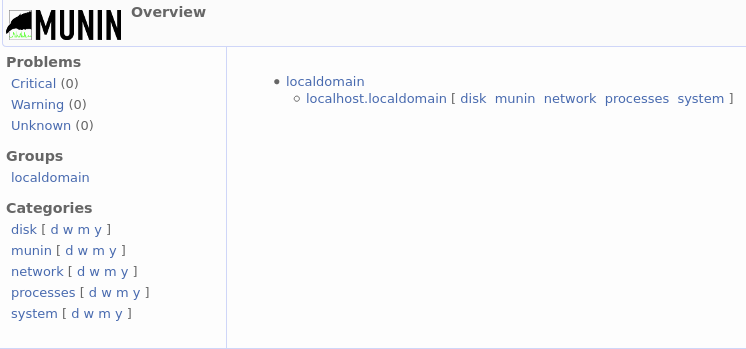
\includegraphics[width=\linewidth]{munin-01.png}
\end{tcolorbox}


\section{Configuración}

Tras la instalación, Munin por defecto tiene una configuración sencilla que hace una monitorización básica del servidor. La configuración se puede encontrar en  \configdir{ /etc/munin/ }   y podemos diferenciar 3 ficheros/directorios:

\begin{itemize}
    \item \textbf{munin.conf}: fichero de configuración principal. En él se puede configurar todo lo relacionado con Munin, avisos, procesos...
    \item \textbf{munin-node.conf}: es el fichero de configuración que se utiliza si se utiliza el sistema básico de monitorización centralizada. En este fichero especificaremos desde qué servidores permitiremos que puedan monitorizar el propio servidor.
    \item \textbf{plugins}: directorio con los plugins activados que se van a utilizar durante la monitorización. En este directorio están los enlaces simbólicos de los plugins que van a ser utilizados durante la monitorización del servidor. Los plugins están en  \configdir{ /usr/share/munin/plugins/ }  . Normalmente suelen ser scripts en los lenguajes Perl, Python o Shell.
\end{itemize}

\section{CRON}

La monitorización del servidor se realiza a través de un proceso CRON que instala Munin y que por defecto se hace cada 5 minutos. El fichero CRON está situado en \configfile{ /etc/cron.d/munin }, y cuenta con 4 procesos automáticos que se ejecutan en el servidor:

\begin{itemize}
    \item Proceso de monitorización
    \item 3 procesos de limpieza de caché y ficheros temporales que son creados durante la monitorización
\end{itemize}


\clearpage